% figures/ch03-genus-vs-N.tex
% Bar chart for genus g(X_0(N)), N=1,...,20
\begin{figure}[ht]
\centering
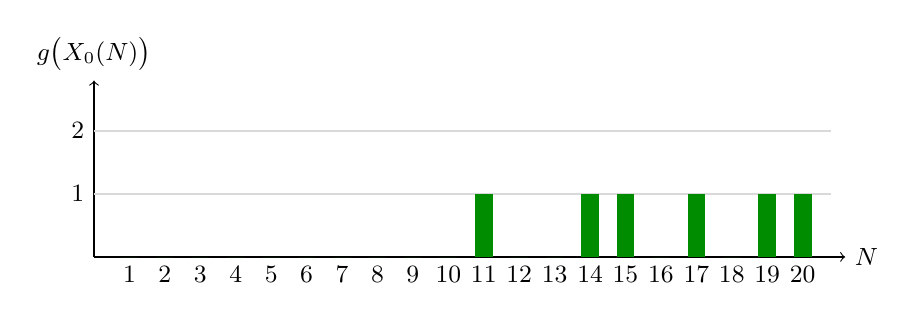
\begin{tikzpicture}[x=0.45cm,y=0.8cm,font=\small]
  \draw[->] (0,0) -- (21.2,0) node[right] {$N$};
  \draw[->] (0,0) -- (0,2.8) node[above] {$g\bigl(X_0(N)\bigr)$};

  \foreach \n in {1,...,20}
    \node[below] at (\n,0) {\n};
  \foreach \y in {1,2}
    {\draw[gray!30] (0,\y) -- (20.8,\y); \node[left] at (0,\y) {\y};}

  \foreach \n/\g in {1/0,2/0,3/0,4/0,5/0,6/0,7/0,8/0,9/0,10/0,11/1,12/0,13/0,14/1,15/1,16/0,17/1,18/0,19/1,20/1}
    \fill[green!55!black] (\n-0.25,0) rectangle (\n+0.25,\g);
\end{tikzpicture}
\caption{$X_0(N)$ 的亏格在小级别的分布。直到 $N=10$ 都还是亏格 $0$；从 $N=11$ 开始，权 $2$ cusp form 才真正稳定出现。}
\label{fig:genus-vs-N}
\end{figure}
